% 用户/组

\subsection{用户/组}

\subsubsection{用户认证}

\textbf{PBKDF2(Password-Based Key Derivation Function)加密算法}
\par
PBKDF2简单而言就是将salted hash进行多次重复计算,这个次数是可选择的。如果计算一次所需要的时间是1微秒,那么计算1百万次就需要1秒钟。假如攻击一个密码所需的彩虹表有1千万条,建立所对应的表所需要的时间就是115天。这个代价足以让大部分的攻击者忘而生畏。

\indent
而该加密算法在NodeJS标准模块中的crypto模块,方法接受5个参数,如crypto.pbkdf2(pwd, salt, iterations, len, fn),分别代表:明文字符串、随机码salt、迭代次数、字节长度、回调函数。在fn中将会得到随机码值和hash值(暗文)。

\noindent
加密算法的核心代码被封装在了lib/auth/pass模块内,代码如下:

\lstset{language=C}

\begin{lstlisting}[frame=single]
/**
 * Module dependencies
 */
var crypto = require('crypto')

/**
 * Bytesize
 */
var len = 128

/**
 * Iterations. ~300ms
 */
var iterations = 12000

/**
 * Hashes a password with optional 'salt', otherwise
 * generate a salt for 'pass' and
 *   invoke `fn(err, salt, hash)`.
 *
 * @param {String} password to hash
 * @param {String} optional salt
 * @param {Function} callback
 * @api public
 */
exports.hash = function (pwd, salt, fn) {
  if ( 3 == arguments.length ) 
    crypto.pbkdf2(pwd, salt, iterations, len, fn)
  else {
    fn = salt
    crypto.randomBytes(len, function(err, salt){
      if (err) return fn(err)
      salt = salt.toString('base64')
      crypto.pbkdf2(pwd, salt, iterations, len, 
       function(err, hash){
        if (err) return fn(err)
        fn(null, salt, hash)
      })
    })
  }
}
\end{lstlisting}

\noindent
用户信息编码/解码(Encode/Uncode)的核心代码如下:

\lstset{language=C}

\begin{lstlisting}[frame=single]
/**
 * encode a user
 */
function encode(user, fn) {
  hash(user.password, function(err, salt, hash) {
    if (err) {
      return fn(err, null)
    }
    user.salt = salt
    user.hash = hash
    fn(err, user)
  })
}
\end{lstlisting} \clearpage

\lstset{language=C}

\begin{lstlisting}[frame=single]
/**
 * uncode a user
 */
function uncode(user, fn) {
  var __u_ = isExisted(user)
  var pass = encodePassword(user)
  if(!__u_) {
    fn(new Error('cannot find user'))
  }
  hash(pass, __u_.salt, function(err, hash) {
    if (err) return fn(err)
    if (hash == __u_.hash) return fn(null, __u_)
    fn(new Error('invalid password'))
  })
}
\end{lstlisting}

\indent
在uncode(user, fn)内的实现代码中,使用到了两个未显示的函数:isExisted(user)和encodePassword(user),其用途分别是判断一个用户是否存在,与对密码进行编码。

\textbf{用户认证机制}
\par
系统在启动服务器后,优先从数据库中读取所有的用户信息,并通过flashDB这么一个缓存管理器,写入到内存中。 \clearpage

\lstset{language=C}

\begin{lstlisting}[frame=single]
/**
 * ready workers
 */
function ready() {
  db.collection('users').find().forEach(
   function(user) {
    utils.encode(user, function(err, user) {
      users.add(user)
    })
  })
}
\end{lstlisting}

\indent
这么做有效利用了局部性原理(缓存),以提高在进行用户认证时的用户体验,在提速的同时,也大大简化了用户认证的业务逻辑,如下代码:

\lstset{language=C}

\begin{lstlisting}[frame=single]
utils.uncode(user, function(err, user) {
  if (!err) {
    // Authentication success !
  }
})
\end{lstlisting}

\indent
另外,这种采用in-memory方式实现用户认证的机制将适时地增加其安全性,它在向服务器中写入用户数据时,将会对每一个对象进行过滤以及增添,例如添加salt值、转换hash值等。


% 发布平台

\subsection{报刊发布平台}
报刊发布平台模块用于提供给高级(企业级)用户定期或不定期发布其电子刊物(副刊)的平台,同时也作为系统管理员/操作员发布主刊的主要用户接口。其功能的特殊性,使得这一平台会频繁地修改服务器数据,相对业务逻辑也比较复杂,因此对前端和后端的性能要求都相对较高。

\begin{figure}[h]
	\centering
		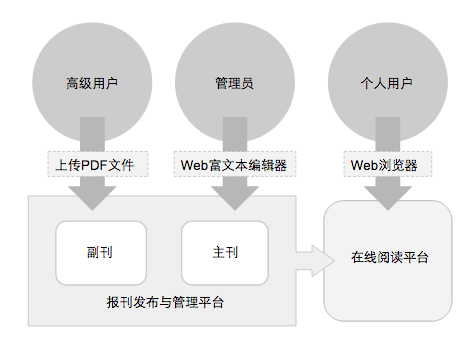
\includegraphics[width=0.8\textwidth]{./images/data-stream-graph.png}
	\caption{报刊发布与管理平台}
\end{figure}

\noindent
为了简化该平台用户发布的操作流程:
\begin{description}
	\item[高级用户] 上传期刊(Issue)的pdf格式的方式来简化流程,通过这种方式来对相应副刊进行管理,可大大简化了高级用户的使用成本;
	\item[管理员] 通过系统基于百度的开源项目Ueditor的Web富文本编辑器来对主刊进行管理;
	\item[个人用户] 我们提供的在线阅读器兼容主流的现代浏览器,相关内容在下一小节中详细说明;
\end{description}

\subsubsection{PDF上传组件}
我们使用了著名开源框架swfupload来为我们提供客户端上传功能,其特点是:多队列上传、类Ajax的用户体验、兼容性良好、灵活自由。它不同于其他基于Flash构建的上传工具,它有着优雅的代码设计,开发者可以利用XHTML、CSS和JavaScript来随心所欲的定制它在浏览器下的外观;它还提供了一组简明的JavaScript事件,借助它们开发者可以方便的在文件上传过程中更新页面内容来营造各种动态效果。

\paragraph{与seajs兼容}
与swfupload官方示例所不同的是,在我们的系统中,需要使用seajs来对swfupload.js文件进行异步加载,不过这也并不困难,只需像下面这样:

\lstset{language=c}

\begin{lstlisting}[frame=single]
seajs.use(['lib/swfupload'], function() {
	var swfu = new SWFUpload({
		'upload_url': 'url replace'
	})
})
\end{lstlisting}

\paragraph{客户端实现}
swfupload提供了一组简明的Javascript事件,下面分别看看常用的几个事件:
\begin{description}
	\item[swfupload\_loaded\_handler()] 在swfupload载入后触发,通常用来对UI进行一些初始化的工作
	\item[file\_dialog\_start\_handler()] 在每次打开选择文件对话框时触发
	\item[file\_queued\_handler(file)] 在成功将一个文件添加到上传等待队列后触发
	\item[file\_queue\_error\_handler(file, err, msg)] 在添加一个文件到队列失败时触发
	\item[file\_dialog\_complete\_handler(fileId, queneId, length)] 确认选择文件对话框后触发,若点击取消并不会触发该事件
	\item[upload\_start\_handler(file)] 上传开始时触发
	\item[upload\_progress\_handler(file, curr, total)] 实时监听上传进度,直到上传完成,其中file为文件对象,curr为已上传的大小,total为总共需要上传的大小,在使用进度条时,会使用到这一事件
	\item[upload\_success\_handler(file, json, res)] 上传成功后触发
\end{description}

\noindent
首先需要在file\_dialog\_complete\_handler事件中执行如下代码:

\lstset{language=c}

\begin{lstlisting}[frame=single]
...
dialogComplete: function(fileId, queuedId, length) {
	this.startUpload()
},
...
\end{lstlisting}

\indent
只有在调用了this.startUpload()这个方法后,才会触发那些与上传相关的事件。

\paragraph{服务端实现}
我们在NodeJS服务器上开放上传功能的接口相对简单,借助于express的bodyParser插件,我们轻松地可以将上传地文件都先缓存到assets/photos/tmp内,然后再根据请求头或请求参数决定如何处理这些文件,并且之后的处理并不阻塞当前请求的返回,从而提高web用户体验。

% 在线阅读

\subsection{在线阅读平台}
该平台提供给个人用户,进行报刊浏览、检索等功能,目标是兼容个大主流的浏览器平台(IE8+,chrome,firefox,safri,opera),由于主刊与副刊格式与显示方式不同,我们将其分开进行说明。

\subsubsection{主刊}
主刊刊主作为系统管理员,是作为所有副刊的索引,也是综合类型刊物最大的报刊,主刊文章是基于HTML编写,因此可以很轻松地展现在阅读器中。

\subsubsection{副刊}
为了简化副刊的发布流程,特意使用了通过上传PDF文件的格式来对其进行最简化,而对于副刊的阅读来说,一个前端性能良好,体验绝佳的PDF阅读器(解析器)是系统所需要的。项目使用了Mozilla的开源项目pdf.js来提供这一功能模块,而将它无缝地嵌入到系统中,也就成为了一个设计重点,好在pdf.js提供了一系列的Javascript接口来供开发者使用,下面就先介绍一下这个开源项目——pdf.js:

\paragraph{pdf.js} 一款基于HTML5的高效PDF解析器,并且完全不依赖于浏览器的本地援助。它是在Mozilla实验室带动下的社区驱动的开源产品,旨在创建一个基于web标准化技术平台下的PDF解析器和渲染器。

\clearpage


